\documentclass[12pt,journal,compsoc, draftclsnofoot,onecolumn]{IEEEtran}

% \usepackage[utf8]{inputenc}
\usepackage{graphicx}

\title{CS 461 - Executive Summary}
\author{Connor Campbell, Chase McWhirt, Jiawei Mo}
\date{December 2018}

\begin{document}

\maketitle

\section{Purpose}
This document is going to cover all important details covered in the problem statement, requirements document, design document, and progress report.
Each will be summarized briefly in its purpose and contents.
This document will also cover the new time line we've created, as well as going into a little bit of depth on the core concepts of the implementation.
Some foreseen issues will also be mentioned with proposed solutions.

\section{The Four Documents}

\subsection{Problem Statement}

The purpose of this document was to clearly define the problem and solution for the entire project.
It has been rewritten to follow the design document more closely.
It also contains updated metrics for the project that should be met.


\subsection{Requirements Document}

This document was also rewritten (mostly) to cover the new plan defined in the design document.
This also contains an updated project time line.
The purpose of this document was define a checklist of goals that must be accomplished for the project to be considered completed.
Since the main point of the project is to implement some method which can dynamically define a mask for objects in a picture in real time, it was difficult to break this down.
The document is now in a decent but partially messy state.
As stated by the instructor, this document is supposed to define the "what" of the project.


\subsection{Design Document}

The design document was a critically important document that defined the planned implementation on a multitude of levels.
It has since clarified the time line and many changes have been made to the project as a result.
As stated by the instructor, this document is supposed to define the "how" of the project.


\subsection{Progress Report}

The purpose of this document was to define the work done in fall term.
It also defined problems the group faced and how they were resolved.
Finally, it restated what the project is and how it is going to be accomplished.
There was difficulty in defining progress since most progress has been writing these documents and completing other class requirements.


\section{New Time Line}

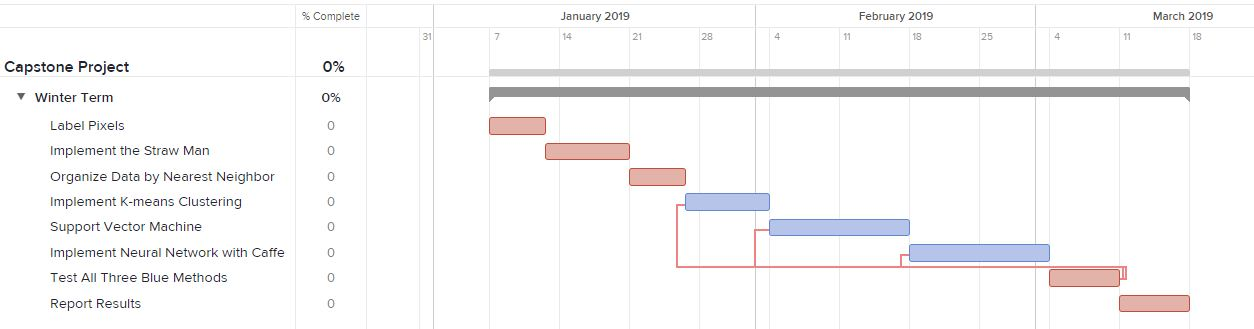
\includegraphics[width=\textwidth]{ganttChart.JPG}

\noindent
This chart depicts our time line for completing the project.
It does not include stretch goals.
We will have a one month that can be used (partially) during Spring term.
However, other assignments for the Capstone project could make using that buffer difficult.


\newpage
\section{Potential Future Issues}

\subsection{Time Line}

\subsubsection{Problem}

It's possible that even this time line is too strict.
It's been designed to be realistically accomplished.
However, unforeseen speed bumps could make it difficult to follow directly.

\subsubsection{Solution}

We'll have weekly check ins to discuss progress.
Each step should take a week so it will be clear when the time line isn't being followed when a step deadline is missed.
It may also be wise to cut one of the implementations such as support vector machines.

\subsection{Group Conflict}

\subsubsection{Problem}

Group conflict may not be an apt name for the problem as a whole, but it does properly identify the most unpleasant symptom.
The root of the problem might be better described in the scenario of an enormous workload constricted to an extremely tight deadline.
It's not fully clear at the time of writing.

\subsubsection{Solution}

There are resources for resolving inter group conflicts in a constructive manner.
This resource specifically allows a moderator to help group member express their anxieties and gripes.
The instructor recommended it early on in the term but the name is unknown at the time of writing.

\noindent
An alternate solution we have already discussed is having weekly group meetings for planning.
This will likely be good anyways as there will need to be coordination to complete each weekly step.
However, unless the root problem is a bad schedule and this solution fully resolves that, it's possible this will only be a temporary measure.


\end{document}
